%&"../virtual"

\begin{document}
    \title{虚拟机安装}
    \maketitle
    \section*{要求}
    Install VMware and create a VM with a different OS.
    \section*{过程}
    安装 VMware Workstation Pro 16.0。相较于 15.5,该版本对实现重写,能够在 Windows 10 的 Hyper-V 功能打开的情况下,启动虚拟机而不会产生冲突,这对于还需要使用 WSL (Windows Subsystem for Linux) 的用户比较友好。
    \begin{figure}[h]
        \centering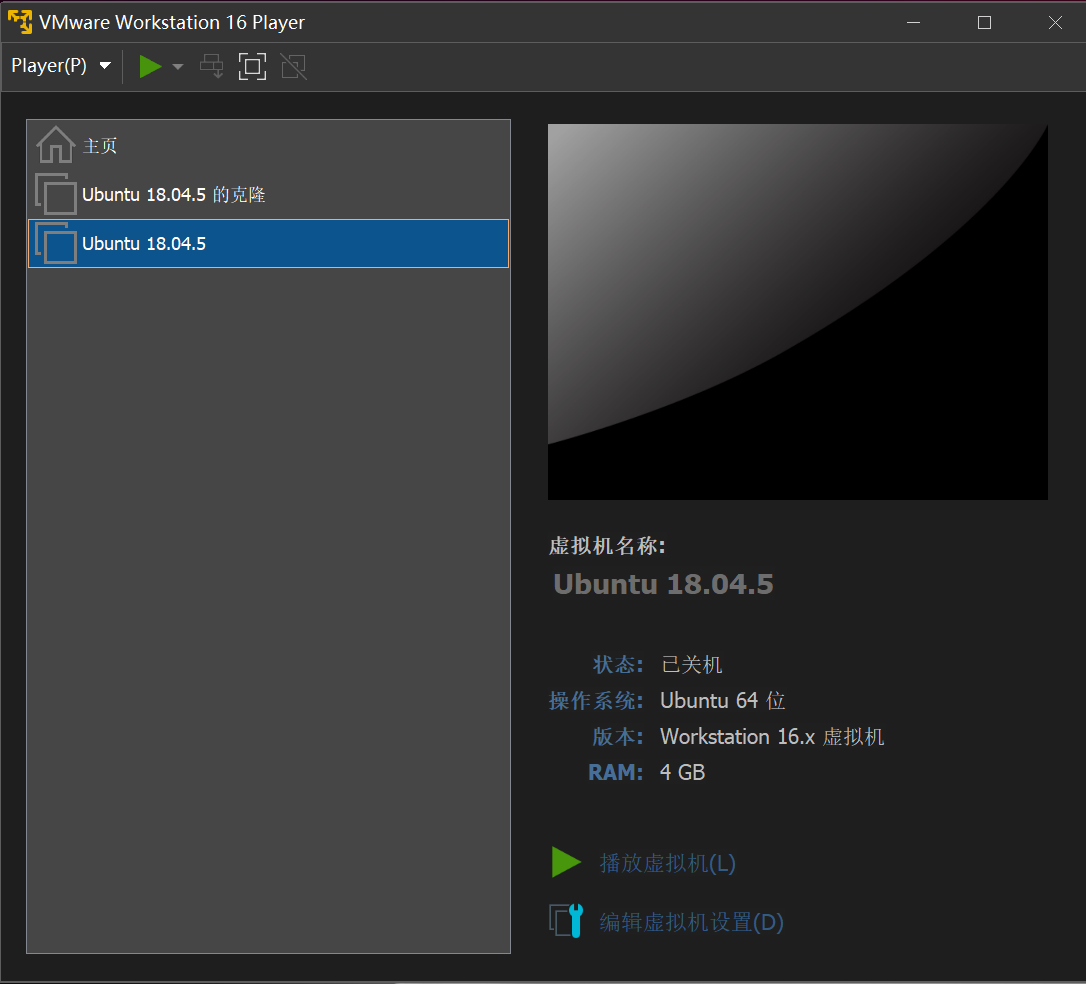
\includegraphics[width=0.6\linewidth]{vmplayer}
        \caption{VMware Workstation 16 Player 界面}
    \end{figure}

    安装 Ubuntu 18.04.5,运行虚拟机。
    \begin{figure}[h]
        \centering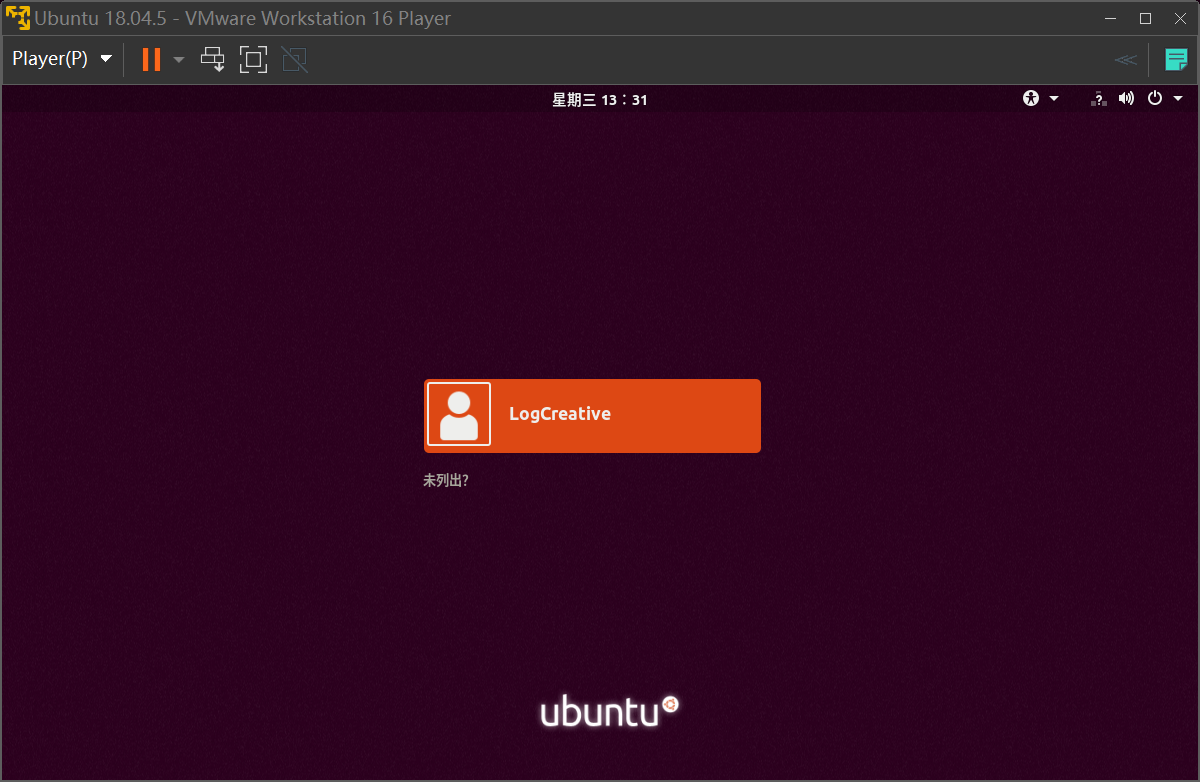
\includegraphics[width=0.6\linewidth]{login}
        \caption{Ubuntu 18.04 登录界面}
    \end{figure}
    \begin{figure}[h]
        \centering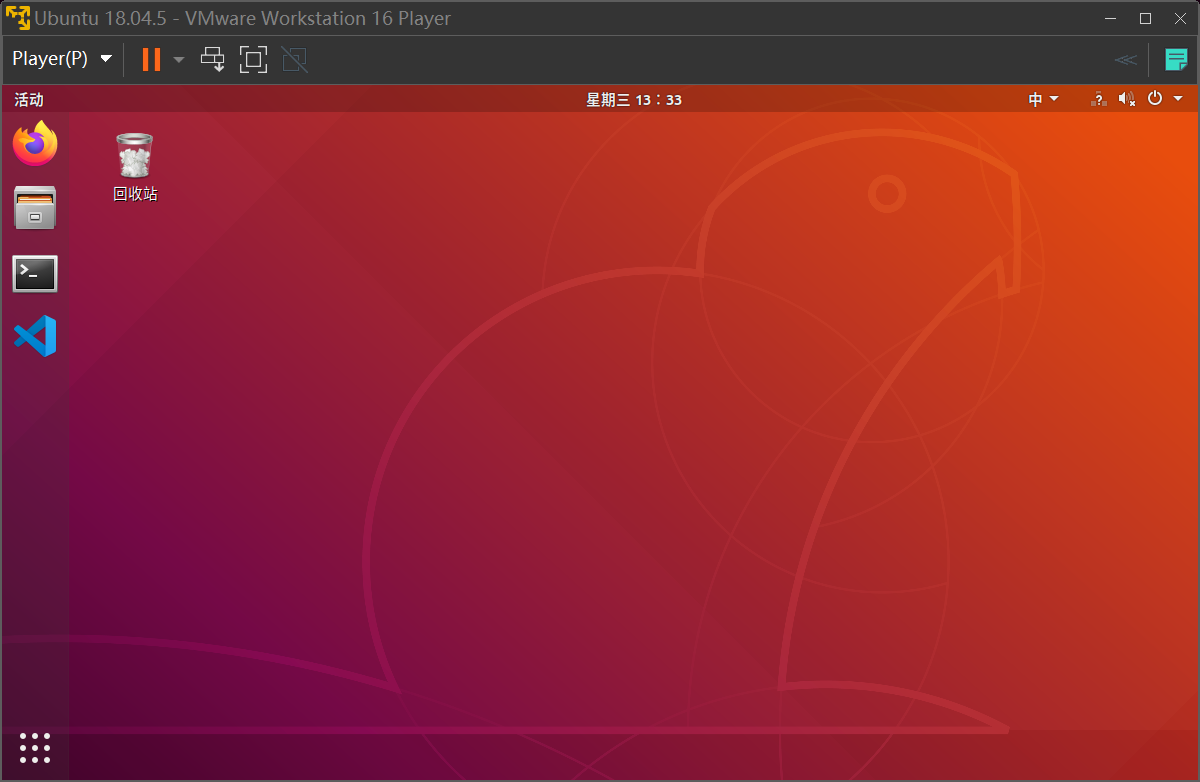
\includegraphics[width=0.6\linewidth]{desktop}
        \caption{Ubuntu 18.04 桌面}
    \end{figure}
    
\end{document}